\subsection{Sensing Subsystem}
\begin{figure}[H]
    \caption{Sensing subsystem block diagram}
    \centering
    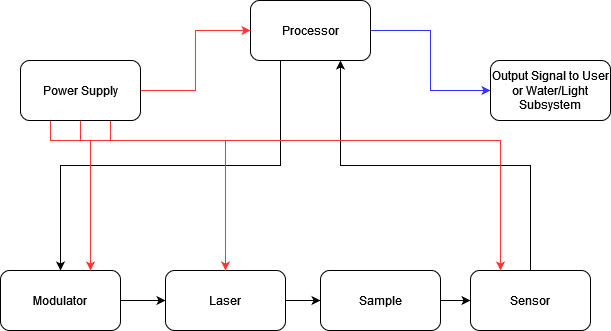
\includegraphics[width=\textwidth]{images/IRSensorBlockDiagram.png}
\end{figure}


The purpose of the Sensing subsystem is to generate a spectrograph of the soil through data delivered to the MCU. Then the MCU will interpret the wavelengths by measuring the amplitude of the signal at several key frequencies. This will determine whether the MCU will proceed to engage the Power and Web subsystems to modify the environment of the plant.


\begin{figure}[H]
    \caption{Photodiode Signal Filter}
    \centering
    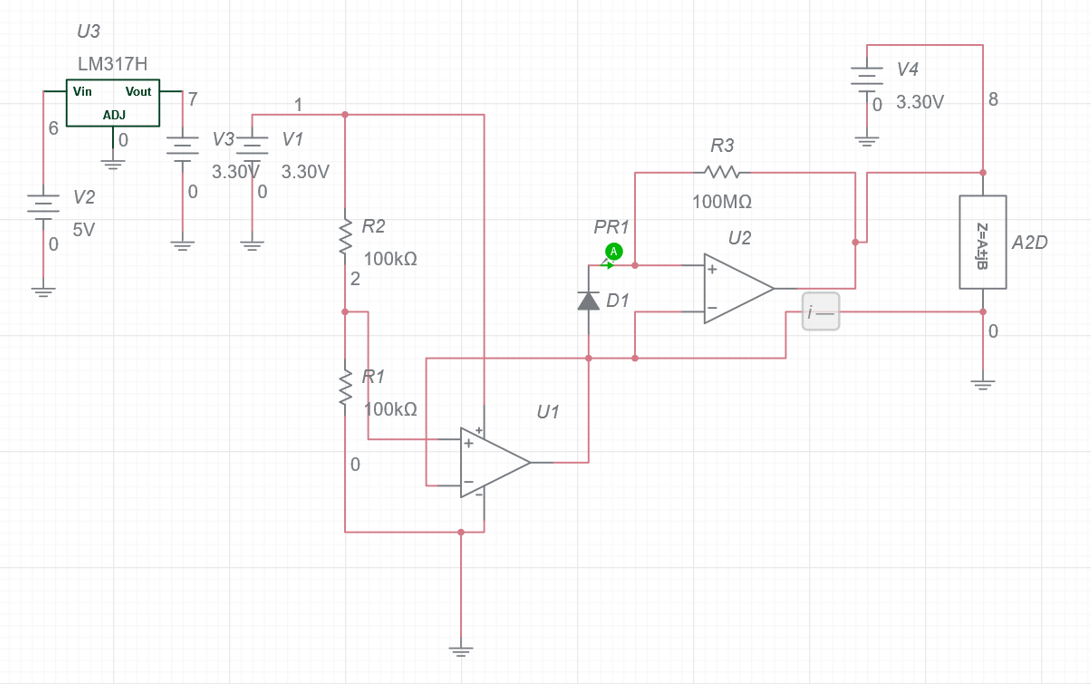
\includegraphics[width=\textwidth]{images/ElectricalSignalFilteringSD1.png}
\end{figure}


The Photodiode works by converting a small portion of the incident light into electrical current across the face of the semiconductor. The diode will have a small current running through the circuit hooked up to an amplifier for boosting the signal to a detectable level. Then another op amp will cut out the electrical noise created by unwanted frequencies generated by the diode and electromagnetic interference.

